\documentclass[tikz]{standalone}
\usepackage{pgfplots}
\usepgfplotslibrary{groupplots}
\def\mfigwidth{14.5}
\def\mradius{1.45}
\def\mmargin{0.35}
\def\mhbcolor{red!60}
\def\mbicarcolor{blue!60}
\def\mdisscolor{gray!60}
\pgfplotsset{width=\mfigwidth, height=7cm, compat=1.18}
\usepackage{tikz}
\usepackage{gensymb}
\usepackage{amsmath}
\usepackage{pgf-pie}
\usetikzlibrary{matrix}

\tikzset{tight matrix/.style={every outer matrix/.append style={inner sep=+0pt}}}

\begin{document}
	% Ok, the code for this figure is overly complicated, and I spent two hours of my life writing it, which was waaaaay too much. All that because I wanted custom legend positioning, which the pgf-pie package does not provide. Also margins in the matrix envs were too big, but changing "inner sep = 0pt" not only changes the outer margins, but also the inner ones - i.e. between nodes. Bref. S0meb0d1 k1ll m3 pliz.
	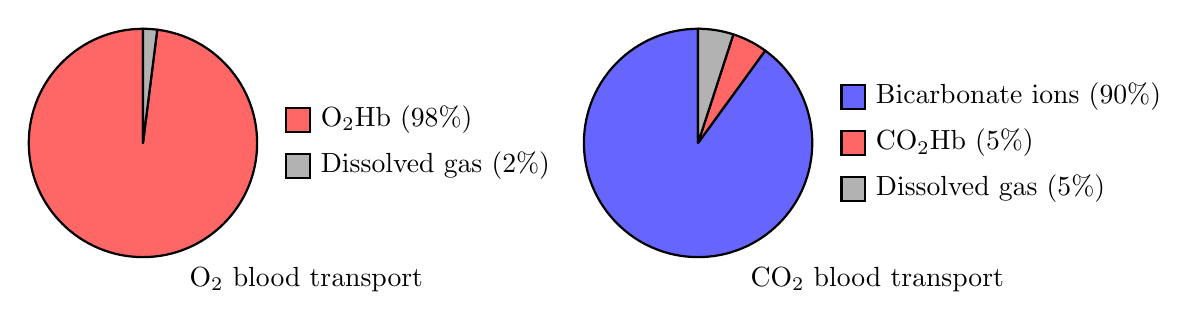
\begin{tikzpicture}
		\pie [pos={\mradius,\mradius}, rotate = 90, radius=\mradius, /tikz/nodes={text opacity=0,overlay}, color={\mhbcolor, \mdisscolor}]
		{98, 2}
		\matrix [right, tight matrix] at (2*\mradius+\mmargin,\mradius) {
			\node[fill=\mhbcolor, thick, draw, minimum height=0.3cm, minimum width=0.3cm, label=right:{O$_2$Hb (98\%)}] at (0,0) {};\\
			\node[fill=\mdisscolor, thick, draw, minimum height=0.3cm, minimum width=0.3cm, label=right:{Dissolved gas (2\%)}] at (0,0) {};\\
		};
		\draw ({(\mfigwidth/2-0.2)/2}, 0) node[below]{O$_2$ blood transport} ;
		\pie [pos={\mfigwidth/2+\mradius-0.20,\mradius}, rotate = 90, radius=\mradius, /tikz/nodes={text opacity=0,overlay}, color={\mbicarcolor, \mhbcolor, \mdisscolor}]
		{90, 5, 5}
		\matrix [right, tight matrix] at (\mfigwidth/2+2*\mradius+\mmargin-0.20,\mradius) {
			\node[fill=\mbicarcolor, thick, draw, minimum height=0.3cm, minimum width=0.3cm, label=right:{Bicarbonate ions (90\%)}] at (0,0) {};\\
			\node[fill=\mhbcolor, thick, draw, minimum height=0.3cm, minimum width=0.3cm, label=right:{CO$_2$Hb (5\%)}] at (0,0) {};\\
			\node[fill=\mdisscolor, thick, draw, minimum height=0.3cm, minimum width=0.3cm, label=right:{Dissolved gas (5\%)}] at (0,0) {};\\
		};
		\draw ({\mfigwidth/2-0.2 + (\mfigwidth/2+0.2)/2}, 0) node[below]{CO$_2$ blood transport} ;
		% Outer Bounding box
		% \draw[draw=black] (0,0) rectangle ++(\mfigwidth, 2*\mradius);
	\end{tikzpicture}
\end{document}
